\section{The Large Hadron Collider}

The Large Hadron Collider (LHC) is the accelerator and collider of circulating beams of protons
or lead ions. 
It sits beneath the French-Swiss border outside of Geneva, in the tunnel that was originally used
for Large Electron-Positron collider (LEP).
 The LHC consists of two beam pipes which house counter-circulating beams and are
merged in four sections around the ring to enable collisions of the beams. Each interaction point
houses a large detector; the layout is shown in Figure \ref{fig:lhc}.

\begin{figure}[htbp]
\centering
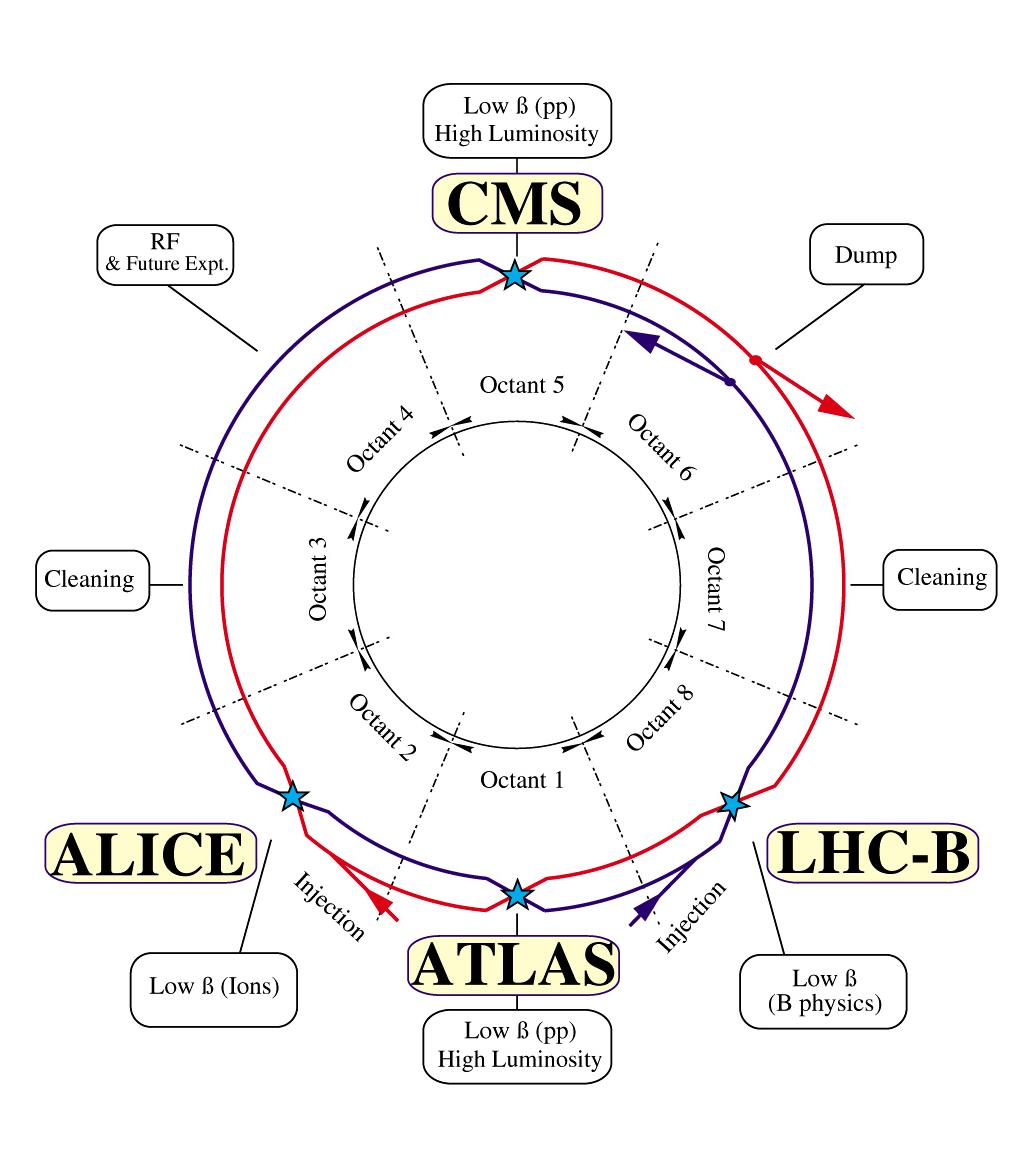
\includegraphics[width=0.5\textwidth]{plots/intro/lhc.jpg}
\caption{The layout of the LHC.\label{fig:lhc}}
\end{figure}

The protons that collide in the LHC are ionized hydrogen atoms which are bunched in groups
of approximately 1.5e11 protons per bunch.
At the first stage, a linear accelerator, Linac2, pushes the protons
 to an energy of 50 \MeV with its electric field. 
From this stage onwards, the protons are accelerated in circular accelerators
using alternating electromagnetic fields at radio frequencies. 
After leaving Linac2 the bunches are injected into the Proton Synchrotron
Booster (PSB) where the protons are accelerated to 1.4 \GeV. 
The next steps are the Proton Synchrotron (PS)
and Super Proton Synchrotron (SPS), which further accelerate the protons
 to 25 and 450 \GeV, respectively.

After the SPS, the proton bunches are injected into the LHC ring, 
where they are accelerated to their
final energy of 4\TeV. The beams are steered through the LHC 
using a series of 1232 superconducting dipole magnets with magnetic fields 
of up to 5.5 Tesla. In order to provide superconductivity the 
dipoles are kept at 1.9 $K$ using superfluid helium.
In addition to the dipoles, there are 400 quadrupole magnets used
for focusing the beams.

The center of mass collision energy for which the LHC was designed, namely 14 \TeV,
 is planned to be achieved in 2015.
In 2012 the LHC operated at a reduced energy of 4 \TeV per proton
and therefore colliding protons at the
center of mass energy $\sqrt{s} = 8 \TeV$.

The instantaneous luminosity of the machine, \ie the rate of scattering events produced divided
by the cross section of the process, is given by:
\begin{equation}
\mathcal{L}=\frac{f n_b N_p^2}{A_{eff}}
\end{equation}
where $f$ is the orbit frequency ($\sim$11 kHz), $n_b$ is the number of colliding bunch pairs, 
$N_p$ is the number of protons per bunch, and $A_{eff}$ is the area in which the bunches
overlap, transverse to the beam directions.


\begin{figure}[htbp]
\centering
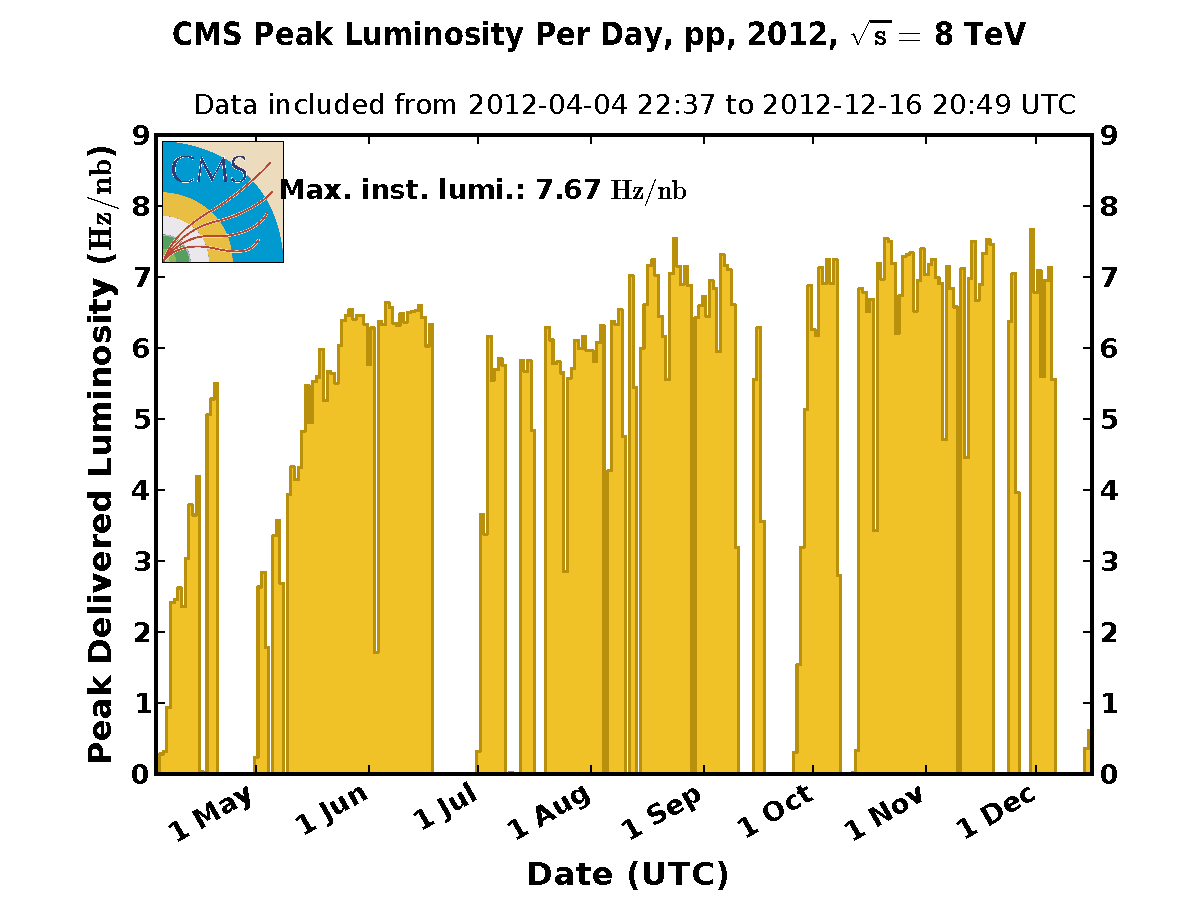
\includegraphics[width=0.49\textwidth]{plots/intro/peak_lumi.pdf}
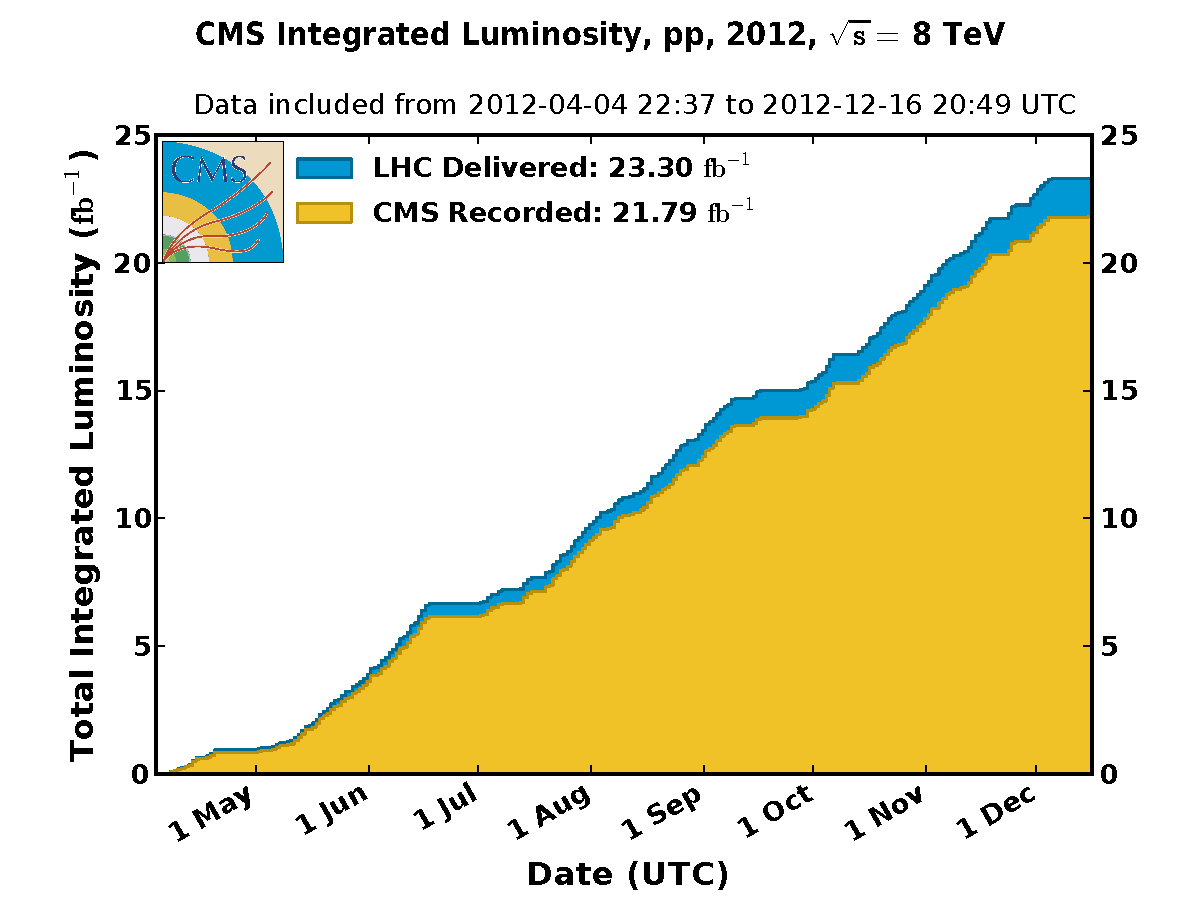
\includegraphics[width=0.49\textwidth]{plots/intro/int_lumi.pdf}
\caption{The daily peak instantaneous luminosity (left) and the integrated luminosity (right)
 delivered to the CMS experiment during the 2012 8\TeV proton-proton run.\label{fig:lumi}}
\end{figure}

The peak instantaneous luminosity delivered to CMS during the 2012 LHC run, 
 reaches 7 $Hz/\mu b$, Figure \ref{fig:lumi}. 
It can be translated to $\sim$30 simultaneous hard scattering interactions 
for each 
crossing of the proton bunches. Simultaneous presence of multiple proton-proton ($pp$) interactions
 poses a significant challenge to the event reconstruction. The total integrated luminosity 
for the 2012 LHC run of 22 \fbinv is the highest integrated luminosity for a hadron collider 
to date.
